% siminos/reversal/JacobianOrb.tex      pdflatex LC21; bibtex LC21
% temporary: siminos/spatiotemp/chapter/LC21JacobianOrb.tex
% $Author: predrag $ $Date: 2021-12-24 01:25:20 -0500 (Fri, 24 Dec 2021) $

\section{Orbit stability}
\label{s:JacobianOrb}

The {temporal lattice} reformulation gives us deep insights into how to
enumerate and determine all global solutions ({\lattstate}s) of
lattice field theories.

The discretized Euler–\-Lagrange
$F[\Xx_c]=0$ fixed point condition \refeq{LC21eqMotion} is central to the
theory of {global methods} for finding periodic orbits. Instead of
utilizing local, forward-in-time numerical integrations, in
global multi-shooting,
collocation\rf{auto,GM00aut,ChoGuck99}, and Lindstedt-Poincar{\'e}\rf{DV02,DV03,DV04}
searches for \po s, one discretizes a \po\ into $\cl{}$
segments\rf{CvitLanCrete02,lanVar1,DingCvit14,DCTSCD14} temporal lattice
configuration,
and lists the field value at a point of each segment
\beq
\transp{\Xx}=(\ssp_0,\ssp_{1},\cdots,\ssp_{\cl{}-1})
\,.
\ee{nXdCycle}
Starting with an initial guess for \Xx, the zero of function
$F[\Xx_c]$ can then be found by Newton iteration, which requires
an evaluation of the $[\cl{}\!\times\!\cl{}]$ \emph{\jacobianOrb}
\beq
\jMorb_{\zeit\zeit'} =\frac{\delta F[\Xx_c]_\zeit}{\delta \ssp_{\zeit'}}
\,.
\ee{jacobianOrb}

\subsection{Temporal Bernoulli, {\templatt}} % \jacobianOrb}
\label{s:JacobianOrbBern}
% joined with \subsection{{\tempLatt} \jacobianOrb}
% \label{s:tempCatJacobianOrb}

The {temporal Bernoulli} condition
\refeq{tempBern} and
the
{\templatt} discretized Euler–\-Lagrange equation \refeq{catTempLatt}
can be viewed as searches for zeros of the vector of
$\cl{}$ functions
\bea
F[\Xx_\Mm] &=& \jMorb\Xx-\Mm = 0
                \label{tempFixPoint}\\
&& \mbox{temporal Bernoulli: } \qquad \jMorb =  - {\shift} + {s}\id
                \label{bernFixPoint}\\
&& \mbox{\templatt: } \qquad\qquad\;\;\,    \jMorb =  -\shift + s\id - \shift^{-1}
                \label{tempCatFix}
\,,
\eea
with the entire periodic \emph{{\lattstate}} ${\Xx}_{\Mm}$ treated as a
single fixed \emph{point} $(\ssp_0,\ssp_{1},\cdots,\ssp_{\cl{}-1})$ in the
\cl{}\dmn\ \statesp\ unit hyper-cube $\Xx\in[0,1)^\cl{}$, and
the $[\cl{}\!\times\!\cl{}]$ {\jacobianOrb}  $\jMorb$.

The $[\cl{}\!\times\!\cl{}]$ {\jacobianOrb} $\jMorb$ is a
%tri-diagonal
Toeplitz matrix, \ie, matrix constant along each diagonal,
$\jMorb_{k\ell} = j_{k-\ell}$, of circulant form,
for the {temporal Bernoulli},
\beq
\jMorb %  = \shift - s\id + \shift^{-1}
  =
\left(\begin{array}{ccccccc}
{s}&-1 & 0 & 0 &\dots &0        & 0 \\
0 & {s}&-1 & 0 &\dots &0        & 0 \\
0 & 0 & {s}&-1 &\dots &0        & 0 \\
\vdots & \vdots&\vdots & \vdots & \ddots &\vdots &\vdots\\
 0 & 0 & 0     & 0     &\dots   & {s}&-1 \\
-1 & 0 & 0     & 0     &\dots& 0& {s}
        \end{array} \right)
\,.
\ee{bernJacOrb}
and for \templatt
\beq
\jMorb %  = \shift - s\id + \shift^{-1}
  =
\left(\begin{array}{ccccccc}
{s}&-1 & 0 & 0 &\dots &0&-1 \\
-1 & {s}&-1 & 0 &\dots &0&0 \\
0 &-1 & {s}&-1 &\dots &0 & 0 \\
\vdots & \vdots &\vdots & \vdots & \ddots &\vdots &\vdots\\
 0 & 0 & 0     & 0      &\dots  & {s}&-1 \\
-1 & 0 & 0     & 0      &\dots&-1 & {s}
        \end{array} \right)
\,.
\ee{Hessian}

\subsection{Nonlinear field theories}
\label{s:henlattJacobianOrb}
%%%%% siminos/kittens/cat.tex                    2021-04-27 %%%%%

The key to understanding their chaoticity are the eigenvalues of
the {\jacobianOrb}, the matrix of second variations of
the action $S[\Xx]_{\zeit\zeit'}$,
%
\beq
\jMorb[\Xx] =
\left(\begin{array}{ccccccc}
%\begin{pmatrix}
 {s}_{0} &-1 & 0 & 0 & \cdots & 0 &-1 \\
-1 & {s}_{1} &-1 & 0 & \cdots & 0 & 0 \\
0 &-1 & {s}_{2}  &-1 & \cdots & 0 & 0 \\
\vdots & \vdots & \vdots & \vdots & \ddots & \vdots & \vdots \\
0 & 0 & 0 & 0 & \cdots & {s}_{\cl{}-2} &-1 \\
-1 & 0 & 0 & 0 & \cdots & -1 & {s}_{\cl{}-1}
%\end{pmatrix}
          \end{array} \right)
\,,
\ee{jMorb1dFT} %was {jMorb1dField}, {PCJiKoKr20(8)}
%
evaluated on a {\lattstate} \Xx,
and its {\HillDet} $\Det\jMorb[\Xx]$,
with the `stretching factor' ${s}_{\zeit}= V''(\ssp_{\zeit})$ at
lattice site $\zeit$ in general a function of the site field $\ssp_\zeit$
for the given \lattstate\ $\Xx$.
    \PC{2020-06-01}{
Cite Gade and Amritkar\rf{GadAmr93} as an early investigation of a
lattice {\jacobianOrb}. They did not know about `Hill's formula.
    }

The {\em \jacobianOrb} is the $\delta/\delta\ssp_k$ derivative of the
{\henlatt} 3-term recurrence relation \refeq{jMorb1dFT}
\bea
\jMorb_p &=& - \shift + 2\,{\mathbb{X}}_p - \shift^{-1}
\,,
\label{Henlatt-orbitJac}
\eea
where ${\mathbb{X}}_p$ is a diagonal matrix with $p$-{\lattstate} $\ssp_k$ in the
$k$th row/column, and the `$1$'s in the upper right and lower left corners
enforce the periodic boundary conditions.

The action of the \henlatt\ {\jacobianOrb} can be hard to visualize,
as a period-2 {\lattstate} is a 2-torus,
period-3 {\lattstate} a 3-torus, \etc. Still, the {\fundPip} for the period-2
and period-3 {\lattstate}s, should suffice to
convey the idea. The {\fundPip} basis vectors \refeq{lattJac} are the
columns of $\jMorb$. The $[2\!\times\!2]$ {\jacobianOrb}
and its {\HillDet} follow from \refeq{Henlatt-2-cycle}
\beq
\jMorb =
 \left(\begin{array}{cc}
2\,\ssp_0   & -2 \\
         -2 & -2\,\ssp_1
 \end{array} \right)
\,,\quad
\Det\jMorb = 4\,(\ssp_0\ssp_1-1)
           = -4\,(a-3)
\,.
\ee{Henlatt-catFundPar2}
% $( 1+ \sqrt{a-3} )( 1- \sqrt{a-3} )-1 = -a+3$
The resulting {\fundPip} shown in \reffig{fig:Henlatt-catCycJacob}\,(a).
Period-3
{\lattstate}s for $s=3$ are contained in the half-open {\fundPip} of
\reffig{fig:Henlatt-catCycJacob}\,(b),
defined by the columns of $[3\!\times\!3]$
{\jacobianOrb}
\beq
\jMorb =
\left(
\begin{array}{ccc}
2\,\ssp_0 &-1           &-1 \\
         -1 & 2\,\ssp_1 &-1 \\
         -1 &-1           & 2\,\ssp_2
\end{array}
\right)
\,,
\qquad
\Det \jMorb
    = 8\,\ssp_0\ssp_1\ssp_2-2\,(\ssp_0+\ssp_2+\ssp_3)+2
\,,
\label{Henlatt-catFundPar3}
\eeq

\subsection{Fundamental fact} %{Integer lattices}
\label{sect:fundFact}

The {\jacobianOrb} \jMorb\ stretches the \statesp\ unit hyper-cube
$\Xx\in[0,1)^\cl{}$ into the \cl{}\dmn\ {\em \fundPip}, and maps each
periodic point ${\Xx}_{\Mm}$ into an integer lattice $\integers^\cl{}$
site, which is then translated by the winding numbers $\Mm$ into the
origin, in order to satisfy the fixed point condition
\refeq{tempFixPoint}. Hence $N_\cl{}$, the total number of the solutions
of the fixed point condition equals the number of integer lattice points
within the {\fundPip}, a number given by what Baake \etal\rf{BaHePl97}
call the \emph{`fundamental fact'},
\beq
N_\cl{} = |\Det\jMorb|
\,,
\ee{detBern0}
\ie, fact that the number of integer points in the {\fundPip} is equal to
its volume, or, what we refer to as the `{\HillDet}' below. In two
dimensions this formula is known since 1899 as
\HREF{https://en.wikipedia.org/wiki/Pick\%27s_theorem} {Pick's theorem},
in higher dimensions it was given by Nielsen\rf{Nielsen1920,BBPT75} in
1920, and rederived several times since in different contexts, for
example by Baake \etal\rf{BaHePl97}. For the task at hand,
Barvinok\rf{Barvinok04}
\HREF{http://www.math.lsa.umich.edu/~barvinok/lectures.pdf} {lectures}
offer a clear and simple introduction to integer lattices, and a proof of
\refeq{detBern0}.
% as {theorem 2}.

%%%%%%%%%%%%%%%%%%%%%%%%%%%%%%%%%%%%%%%%%%%%%%%%%%%%%%%%%%%%%%%%%%%%%%%
% BernCyc2Jacob.svg
% derived from CatMapStatesp.svg
\begin{figure}
  \centering
(a)~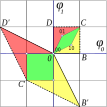
\includegraphics[width=0.35\textwidth]{BernCyc2JacobUnit}
~~~~~~
(b)~\includegraphics[width=0.22\textwidth]{BernCyc2JacobPart}
  \caption{\label{fig:BernCyc2Jacob}
(Color online)~~~
  (a)
The Bernoulli map \refeq{BerShift} periodic points
$\Xx_\Mm=(\ssp_0,\ssp_1)$ of period 2 are the $\cycle{0}=(0,0)$ fixed
point, and the 2-cycle $\Xx_{01}=({1}/{3},{2}/{3})$, see
\reffig{fig:BernPart}\,(a). They all lie within the unit square $[0BCD]$,
which is mapped by the {\jacobianOrb} $\jMorb$ \refeq{bernFundPar} into
the {\fundPip} $[0B'C'D']$. Periodic points $\Xx_\Mm$ are mapped by
$\jMorb$ onto the integer lattice, $\jMorb\Xx_\Mm\in\integers^\cl{}$, and
are sent back into the origin by integer translations $\Mm$, in order to
satisfy the fixed point condition \refeq{tempFixPoint}. Note that this
{\fundPip} is covered by  3 unit area quadrilaterals, hence
$|\Det\jMorb|=3$.
    (b)
Conversely, in the flow conservation sum rule \refeq{H-OdeA_mapsOrb2} sum
over all {\lattstate}s $\Mm$ of period $\cl{}$, the inverse of the
{\HillDet} defines the `neighborhood' of a lattices state as the
corresponding fraction of the unit hypercube volume.
          }
\end{figure}
%%%%%%%%%%%%%%%%%%%%%%%%%%%%%%%%%%%%%%%%%%%%%%%%%%%%%%%%%%%%%%
%
The action of {\jacobianOrb}
$\jMorb$ for the period-2 {\lattstate}s (periodic points) of the Bernoulli map of
\reffig{fig:BernPart}\,(a), suffices to convey the idea. In this
case, the $[2\!\times\!2]$ {\jacobianOrb} \refeq{tempBern}, the unit
square basis vectors, and their images are
\bea
\jMorb &=&
 \left(\begin{array}{cc}
  2 & -1 \\
 -1 &  2
 \end{array} \right)
    \continue
\Xx^{(B)} &=&
 \left(\begin{array}{c}
 1  \\
 0
 \end{array} \right)
\;\to\;
\Xx^{(B')} = \jMorb\,\Xx^{(B)} =
 \left(\begin{array}{c}
  2  \\
 -1
 \end{array} \right)
\,,\quad \cdots
\nnu
\eea
\ie, the columns of the {\jacobianOrb} are the edges of the {\fundPip},
\beq
\jMorb = \left(\Xx^{(B')}\Xx^{(D')}\right)
\,,
\ee{bernFundPar}
see \reffig{fig:BernCyc2Jacob}\,(a), and $N_2=|\Det\jMorb|=3$,
in agreement with the periodic orbit count \refeq{noPerPtsBm}.

In general, the unit vectors of the \statesp\ unit hyper-cube
$\Xx\in[0,1)^\cl{}$ point along the \cl{} axes; {\jacobianOrb} \jMorb\
stretches them into a {\fundPip} basis vectors $\Xx^{(j)}$, each one a
column of the $[\cl{}\!\times\!\cl{}]$ matrix
\beq
\jMorb = \left(\Xx^{(1)}\Xx^{(2)}\cdots\Xx^{(\cl{})}\right)
\,.
\ee{lattJac}
The {\HillDet}
\beq
\Det \jMorb = \Det\!\left(\Xx^{(1)}\Xx^{(2)}\cdots\Xx^{(\cl{})}\right)
\,,
\ee{lattVol}
is then the volume of the {\fundPip} whose edges are basis vectors
$\Xx^{(j)}$. Note that the unit hypercubes and {\fundPip}s are half-open,
as indicated by dashed lines in \reffig{fig:BernCyc2Jacob}\,(a), so that
their translates form a partition of the extended \statesp\
\refeq{BerStretch}. For another example of {\fundPip}s, see
\reffig{fig:catCycJacob}.
% and \refeq{3times2basisVecs}.

Note that in the {temporal lattice} reformulation, the Bernoulli system
involves two distinct lattices:
\begin{itemize}
  \item[(i)]
Any lattice field theory:
in the discretization \refeq{LattField}
 of the time continuum, one replaces \emph{any}
dynamical system's time-dependent field $\ssp(\zeit)\in\reals$ at time
$\zeit\in\reals$ by a discrete set of its values
$\ssp_\zeit=\ssp(a\,\zeit)$ at time instants $\zeit\in\integers$.
Here the index $\zeit$ is a \emph{coordinate} over which the field
$\ssp$ is defined.
  \item[(ii)]
Specific to the Bernoulli system: the site $\zeit$ field value
$\ssp_{\zeit}$ \refeq{n-tuplingMap} is confined to the unit interval
$[0,1)$, imparting integer lattice structure onto the intermediate
calculational steps in the extended \statesp\ \refeq{BerStretch} on which
the {\jacobianOrb} \jMorb\ \refeq{tempBern} acts.
\end{itemize}

    \PC{2021-10-25}{
    Combine the above with the \templatt\ \refpage{} discussion into a
    remark that temporal Bernoulli and \templatt\ aslo have a
    \emph{dynamical} \Dn{1} symmetry, not utilized in this paper, as
    nonlinear field theories such as \henlatt\ do not have such
    symmetries. Here we study only the symmetries of the floor, not the
    dancer.
    }

For \templatt\ the total number of {\lattstate}s is again, as
for the Bernoulli system \refeq{detBern0}, given by the `fundamental
fact \refeq{detBern0}.
However, while for the temporal Bernoulli every sequence of alphabet
letters \refeq{base-sAlph}  but one is admissible, for \templatt\ the
condition \refeq{catMapNewt} constrains admissible source {\brick}s \Mm.

For period-1, constant field  {\lattstate}s
$\ssp_{\zeit+1}=\ssp_{\zeit}=\ssp_{\zeit-1}$
it follows from
\refeq{catMapNewt} that
\[
        ({s}-2)\ssp_\zeit = \Ssym{\zeit}
\,,
\]
so the {\jacobianOrb} is a $[1\times1]$ matrix, and there are
\beq
N_1={s}-2
%\,,
\ee{catFundPar1}
period-1 {\lattstate}s. This is easy to verify by counting the admissible
$\Ssym{\zeit}$ values. Since $\ssp_\zeit \in [0,1)$, the range of
\Ssym{\zeit} is $\Ssym{\zeit} \in [0,s-2)$. So three of the
\refeq{catAlphabet}  \templatt\  letters are not admissible:
$\underline{1}$ is below the range, and $s-2$ and $s-1$ are above it.

%%%%%%%%%%%%%%%%%%%%%%%%%%%%%%%%%%%%%%%%%%%%%%%%%%%%%%%%%%%%%
% Predrag 2020-02-08 replaced Han's
% {HLLength2Counting}.pdf by hand-drawn catCyc2Jacob.svg
% Han & PC 2020-02-11
% siminos/figSrc/han/Mathematica/CountingFigure/HLLength3Counting.nb
\begin{figure}
  \centering
(a)~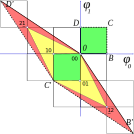
\includegraphics[width=0.38\textwidth]{catCyc2JacobUnit}
~~~
(b)~\includegraphics[width=0.34\textwidth]{PCLength3Counting}
  \caption{\label{fig:catCycJacob}
    (Color online)~~~
(a)
    For $s=3$, the \templatt\ \refeq{catTempLatt} has 5 period-2
    {\lattstate}s $\Xx_\Mm=(\ssp_0,\ssp_1)$: $\Xx_{00}$ fixed point and
    2-cycles $\{\Xx_{01},\Xx_{10}\}$,
    $\{\Xx_{\underline{1}2},\Xx_{2\underline{1}}\}$. They lie
    within the unit square $[0BCD]$, and are mapped by the
    $[2\!\times\!2]$ {\jacobianOrb} $\jMorb$ \refeq{catFundPar2} into the
    {\fundPip} $[0B'C'D']$, as in, for example, Bernoulli
    \reffig{fig:BernCyc2Jacob}. The images of periodic points $\Xx_\Mm$
    land on the integer lattice, and are sent back into the origin by
    integer translations $\Mm= \Ssym{0}\Ssym{1}$, in order to satisfy the
    fixed point condition
    %\refeq{tempFixPoint},
    $\jMorb\Xx_\Mm+\Mm=0$.
(b) A 3-dimensional [{\color{blue} blue} basis vectors] unit-cube stretched by
    $\jMorb$ \refeq{catFundPar3} into the [{\color{red} red} basis vectors]
    {\fundPip}. For $s=3$, the \templatt\
    \refeq{catTempLatt} has 16 period-3 {\lattstate}s: a $\Xx_{000}$
    fixed point at the vertex at the origin, [{\color{red} pink dots}] 3
    period-3 orbits on the faces of the {\fundPip}, and
    [{\color{blue} blue dots}] 2 period-3 orbits in its interior.
    An \cl{}\dmn\ \statesp\ unit hyper-cube $\Xx\in[0,1)^\cl{}$ and the
    corresponding {\fundPip} are half-open, as indicated
    by dashed lines, so the integer lattice points on the far corners, edges
    and faces do not belong to it.
}
\end{figure}
%%%%%%%%%%%%%%%%%%%%%%%%%%%%%%%%%%%%%%%%%%%%%%%%%%%%%%%%%%%%%%%

The action of the \templatt\ {\jacobianOrb} can be hard to visualize,
as a period-2 {lattice field} is a 2-torus,
period-3 {lattice field} a 3-torus, \etc. Still, the {\fundPip} for the period-2
and period-3 {\lattstate}s, \reffig{fig:catCycJacob}, should suffice to
convey the idea. The {\fundPip} basis vectors %\refeq{lattJac}
are the
columns of $\jMorb$. The $[2\!\times\!2]$ {\jacobianOrb} \refeq{Hessian}
and its {\HillDet} are
\beq
\jMorb =
 \left(\begin{array}{cc}
  s & -2 \\
 -2 &  s
 \end{array} \right)
\,,\qquad
N_2=\Det\jMorb=({s}-2)({s}+2)
\,,
\ee{catFundPar2}
(compare with the {\lattstate}s count
\refeq{1stChebGenF}),
with the resulting {\fundPip} shown in \reffig{fig:catCycJacob}\,(a).
Period-3
{\lattstate}s for $s=3$ are contained in the half-open {\fundPip} of
\reffig{fig:catCycJacob}\,(b), defined by the columns of $[3\!\times\!3]$
{\jacobianOrb}
\beq
\jMorb =
\left(
\begin{array}{ccc}
 {s}& -1 & -1 \\
 -1 & {s}& -1 \\
 -1 & -1 & {s}
\end{array}
\right)
\,,
\qquad
N_3 = \Det \jMorb
%   = {s}^3-3{s}-2
    = ({s}-2)({s}+1)^2
\,,
\label{catFundPar3}
\eeq
again in agreement with the periodic orbit count \refeq{1stChebGenF}.
The 16 period-3, ${s}=3$ {\lattstate}s $\Xx_\Mm=(\ssp_0,\ssp_1,\ssp_3)$
are the $\Xx_{000}$ fixed point at the vertex at the origin, 3 period-3
orbits on the faces of the {\fundPip}, and 2 period-3 orbits in its
interior.
    \PC{2021-10-29}{Dropped:
, all five of form
    $\{
       \Xx_{\Ssym{0}\Ssym{1}\Ssym{2}},
       \Xx_{\Ssym{1}\Ssym{2}\Ssym{0}}
       \Xx_{\Ssym{2}\Ssym{0}\Ssym{1}}
    \}$
.
    }

    In this example there is no need to go further with the fundamental
fact \HillDet\ evaluations, as the explicit formula for the numbers
of periodic {\lattstate}s is well known\rf{Isola90,Keating91}.
The \templatt\ equation \refeq{catMapNewt} is
a linear {$2$nd-order inhomogeneous difference} equation
($3$-term recurrence relation) with constant coefficients
that can be solved by standard methods\rf{Elaydi05} that
parallel the theory of linear differential equations.
Inserting a solution of form $\ssp_{\zeit}=\ExpaEig^\zeit$ into the
\Ssym{\zeit}=0 homogenous {$2$nd-order \templatt\ condition}
\refeq{catMapNewt}
yields the {characteristic equation} \refeq{LC21:StabMtlpr}
with roots
$\{\ExpaEig\,,\;\ExpaEig^{-1}\}$.
The result is that the number
of temporal {\lattstate}s of period $\cl{}$ is
\beq
N_{\cl{}}  = |\Det\jMorb| =
    \ExpaEig^{\cl{}} + \ExpaEig^{-\cl{}} - 2
\,,
\ee{1stepDiffSolu}
often written as
\beq
N_\period{}
 = 2\,T_{\period{}}(s/2) -2
% = \ExpaEig^{\period{}} + \ExpaEig^{-\period{}} - 2
\,,
\label{POsChebyshev}
\eeq
where $T_{\period{}}(s/2)$ is the Chebyshev polynomial of the first kind.
% end of copied from siminos/spatiotemp/chapter/Green1d.tex

Note that in the {temporal lattice} reformulation, the \templatt\
happens to involve two unrelated lattices:
\begin{itemize}
  \item[(i)]
In the latticization of a time continuum, one replaces a time-dependent
field $\ssp(\zeit)$ at time $\zeit\in\reals$ of \emph{any} dynamical system by a
discrete set of its values $\ssp_\zeit=\ssp(\zeit\Delta{T})$,
$\zeit\in\integers$. Here the index $`\zeit'$ is a \emph{coordinate} over
which the field $\ssp$ lives.
  \item[(ii)]
A peculiarity of the \templatt\ is that the \emph{field} $\ssp_{\zeit}$
\refeq{eq:StateSpCatMap} is confined to the unit interval $[0,1)$,
imparting a $\integers^1$ lattice structure onto the calculationally
intermediate {\fundPip} $\jMorb$ basis vectors \refeq{lattJac}.
\end{itemize}

\subsection{\JacobianOrb\ on reciprocal lattice}
\label{sect:LC21recip1d} % started with {sect:RhombCornerFT}

    \PC{2021-08-28}{Define the \HillDet\ somewhere, refer to it here.}
we show how compute the {\jacobianOrb} or {\HillDet}s
$|\Det\jMorb|$ using crystallographer's favorite tool, the discrete
Fourier transform.
